% !Mode:: "TeX:UTF-8"

% ---------- 声明文档类 ---------- %
% 有两个可选参数:bachelors、bachelorh
%% bachelors:理工科模式
%% bachelorh:文科模式
% 添加哪个参数即表示选择哪种模式
\documentclass[bachelorh]{dlmubachelorthesis}
% ================================================== %


% --------------- 添加批注 --------------- %
\let\comment\undefined
\usepackage[]{changes}
\definechangesauthor[name={海哥}, color=blue]{海哥} %创建批注者信息
\definechangesauthor[name={海老}, color=red]{海老} %创建批注者信息
% ======================================== %


% -------------------- 填写论文信息 -------------------- %
\cntitle{提高我国医疗保障水平问题研究} %【中文标题】
\entitle{Study on the Issue of Improving the Level of Medical Insurance in China} %【英文标题】
\aauthor{海哥} %【作者姓名】
\sdtID{222020xxxx} %【学号】
\faculty{公共管理与人文艺术学院} %【学院】
\majorinCOVERPAGE{公共事业管理2020-1} %【专业年级班级(coverpage专用)】
\mentorONE{海老}{教授} %【指导教师(及其职称)】
\mentorTWO{无}{0} %【第二指导教师(及其职称)】【若无,则第一个参数填“无”,第二个填数字0】
\completiondate{2024}{5} %【完成日期(年、月)】
% ================================================== %


% ----- 文科类专业专用:脚注编号类型的选择 ----- %
%% 填“1”:仅阿拉伯数字
%% 填“2”:[1], [2], ...
%% 填“3”:(1), (2), ...
%% 填“4”:带圈的阿拉伯数字
\footnotemode{4}
% ============================================= %


% ---------- 可以在此处添加自己定义的命令 ---------- %

% ================================================== %


\begin{document}

\makepages %【添加封面页】

% ---------- 中文摘要 ---------- %
\begin{abstract}

% ---------- 中文摘要内容 ---------- %
{\zihao{-4} %【该句涉及到格式设置,请勿乱动】

医疗保障是社会保障体系的重要组成部分。完善的医疗保障体系是人民群众生活的基本需求,是整个社会正常运转的基础,是经济发展的促进剂,所以提高我国的医疗保障水平是十分必要的。本文依据医疗保障的基本理论,分四部分对我国的医疗保障制度和水平做了系统性的研究。第一部分先是介绍了医疗保障和医疗保障水平的含义,然后从医疗保障在社会中发挥的功能、作用和重要地位三方面阐述了对我国医疗保障水平进行研究的必要性。第二部分对城镇和农村的医疗保障水平进行了具体地介绍,并将两方面进行分析比较,其中对公平性方面做了着重分析,从而综合性地阐述了我国医疗保障制度的现状。第三部分对国外几个比较有代表性的国家英国、德国、美国、新加坡的医疗保障制度进行介绍,并与我国的医疗保障水平比较后总结出适合我国发展的经验。第四部分就未来如何提高我国的医疗保障水平问题提出一些对策和建议。包括社会医疗保险制度的完善与发展,明确基本医疗保障范围,逐步实现覆盖全民一体化医疗保障体制,政府加强医疗保障投入,建立平价医院五方面。


\keywordsCN{医疗保障水平;医疗保障制度;对策}
}


\end{abstract}
\newpage
% ============================== %	


% ---------- 英文摘要 ---------- %
\renewcommand\abstractname{\large ABSTRACT} %临时修改摘要名
\begin{abstract}

% ---------- 英文摘要内容 ---------- %
{\zihao{-4} %【该句涉及到格式设置,请勿乱动】

Medical insurance is one of the important parts of social security system. Prefect medical insurance system is a basic requirement for people’s daily life, an essential element of social common proceeding, an accelerant for economical development. Therefore, the study of our country’s medical insurance level is very necessary.In this paper, based on medical protection of the basic theory, from the four major areas of our country’s level medical insurance system and does a systematic study. The first part introduce the meaning of medical insurance and medical insurance level and then from the medical insurance play in society function, role and important position on the three aspects to study our country's medical insurance level is needed. The second part specific introduces the medical insurance level of the urban and rural, compares the two parts; one of the fair has done a focus on analysis and a comprehensive exposition of our country's medical insurance system for the status quo. The third part introduces the medical insurance system of several foreign countries more representative, Britain, Germany, the United States and Singapore.

\keywordsEN{Medical insurance level; Medical insurance system; Countermeasure}
} 
\end{abstract}
\newpage
% ============================== %


% ---------- 目录 ---------- %
\tableofcontents
\listofchanges
\newpage
% ================================================== %	


\pagestyle{fancy} %从第一章到致谢,设置为有页眉、有页脚的模式
\pagenumbering{arabic} %《手册》要求:从正文开始设为阿拉伯数字页码,并且重新从1开始计数


% ---------- 正文首页标题 ---------- %
\cntitleinMAINBODY %【插入中文标题】
% ================================================== %


% ---------- 正文(划分为多个独立文件依次导入) ---------- %


医疗保障制度是社会保障制度的重要组成部分。完善的医疗保障制度,不仅可以有效的维护社会经济安全、稳定的发展,更重要的是它是促进社会公正、维护公民基本权利的一种重要手段。但是长期以来,我国的医疗保障水平依旧存在着一些的问题。城乡差异较大,公平性有待提高等都是当前摆在我们面前亟待解决的问题。

\section{我国医疗保障水平}

\subsection{医疗保障含义}

医疗保障是指一个社会通过正式的和非正式的制度安排为其公民提供所有健康保障服务的一种社会制度。医疗保障分为广义和狭义两种。“只要我想到我是什么东西,他就永远不能使我成为什么都不是”;“那么我究竟是什么呢?是一个在思维的东西。”\footnote{勒内•笛卡尔.第一哲学沉思录.北京:九州出版社,2007:P43}笛卡尔对“人是什么”这个问题的解答很好地诠释了理性主义在其萌发时期,为理性——即“思”树立为人的唯一本质性存在的基础埋下伏笔。

\subsection{医疗保障对社会发展的作用}

\subsubsection{维护社会稳定}

为减少社会风险,保持社会的稳定发展,通过建立包括医疗保障制度在内的社会保障体系来减轻社会风险对社会稳定造成的冲击\upcite{童星2002},使之成为维护社会稳定的一种“减震器”。

\subsubsection{促进经济发展}

医疗保险的社会化管理,提高了医疗保险基金的共济能力\upcite{郑功成2002},使用人单位能够用较少的费用即能达到保障目的,减轻了企业的负担,有利于推进企业改革的深入和企业的成长壮大。

\subsubsection{调节收入分配}

医疗保险缴费与收入挂钩,不同收入人群缴费不一样,通过医疗保险基金发挥共济作用,从纵向实现调节收入分配功能。参保人员享受相同的保障待遇,体现了横向公平。“我思故我在”,作为古典理性主义哲学理论上的出发点,在意志主义哲学中,被解读为:“思”若是条件,则“我”是受制约的;因此,“我”只是一个综合,此综合是由思本身制造的。\footnote{尼采.论道德的谱系,善恶之彼岸.桂林:漓江出版社,2007:P165.}

\subsection{本章小结}

本章主要介绍了医疗保险的相关知识。医疗保障是指一个社会通过正式的和非正式的制度安排为其公民提供所有健康保障服务的一种社会制度。

 \clearpage\vspace*{0pt} %\vspace*{0pt}的添加解决了章节标题前间距不合理的问题

\section{基础知识}

基于视频序列的运动目标检测与跟踪涉及到很多研究领域,如数字图像处理、计算机视觉、信息融合、模式识别与人工智能等。

\subsection{视频图像预处理}

\subsubsection{常用颜色模型}

颜色模型的用语是在某些标准下用通常可接受的方式简化彩色规范。本质上颜色模型是坐标系统和子空间的规范。位于系统中的每种颜色都由单个点来表示。

(1)~RGB彩色模型:

在RGB模型中,每种颜色出现在红、绿、蓝的原色光谱分量中,这个模型基于笛卡尔坐标系。

图\ref{fig:RGB彩色立方体示意图}所示的立方体。图中R、G、B位于$3$个角上。在该模型中,灰度等级沿着主对角线从原点的黑色到点$(1,1,1)$的白色分布。
\begin{figure}[H]
  \centering
  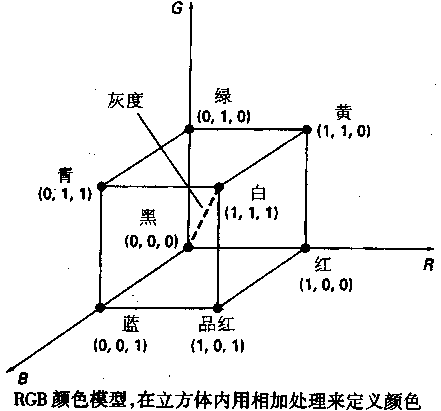
\includegraphics[width=0.45\textwidth]{fig_ch2/RGB彩色立方体示意图.png}
  \caption{RGB彩色立方体示意图}
  \label{fig:RGB彩色立方体示意图}
\end{figure}

(2)~灰色模型:

本质上颜色模型是坐标系统和子空间的规范。位于系统中的每种颜色都由单个点来表示。单位在每列的书写示例如表\ref{tab:单位在每列的书写示例}所示。

\begin{table}[H]
  \centering
  \caption{单位在每列的书写示例}
    \begin{tabular}{ccccc}
    \toprule
    基体 & 序号 & \makecell[c]{粉末类型和\\ 预热温度(\unit{\degreeCelsius})} & 失效温度(\unit{\degreeCelsius}) & $E_c$计算值(\unit{\GPa})\\
    \midrule
    \multicolumn{1}{c}{\multirow{4}[2]{*}{SUS304不锈钢}} & 1     & 粗粉 \& 1000 & 180   & 4.21 \\
          & 2     & 粗粉 \& 800 & 10    & 4.38 \\
          & 3     & 细粉 \& 1000 & 300   & 4.95 \\
          & 4     & 细粉 \& 800 & 120   & 5.08 \\
    \bottomrule
    \end{tabular}%
  \label{tab:单位在每列的书写示例}%
\end{table}%

表格的分栏情况示例如表\ref{tab:分栏情况示例}所示。
% Table generated by Excel2LaTeX from sheet 'Sheet1'
\begin{table}[H]
  \centering
  \caption{分栏情况示例}
    \begin{tabular}{cccc}
    \toprule
    \multicolumn{1}{c}{基体} & 粉末类型 & \multicolumn{1}{c}{预热温度(\unit{\degreeCelsius})} & \multicolumn{1}{c}{平均值} \\
    \midrule
    \multicolumn{1}{c}{\multirow{6}[4]{*}{SUS304不锈钢}} & \multirow{3}[2]{*}{粗粉} & 600   & 44.28\% \\
          & \multicolumn{1}{c}{} & 800   & 42.37\% \\
          & \multicolumn{1}{c}{} & 1000  & 39.74\% \\
\cmidrule{2-4}          & \multirow{3}[2]{*}{细粉} & 600   & 27.95\% \\
          & \multicolumn{1}{c}{} & 800   & 25.41\% \\
          & \multicolumn{1}{c}{} & 1000  & 24.77\% \\
    \midrule
    \multicolumn{1}{c}{\multirow{2}[2]{*}{碳钢}} & 粗粉    & 1000  & 35.65\% \\
          & 细粉    & 1000  & 22.95\% \\
    \bottomrule
    \end{tabular}%
  \label{tab:分栏情况示例}%
\end{table}%

表的通栏情况和全表统一单位的情况如表\ref{tab:插入表格的通栏示例(单位:台)}所示。
% Table generated by Excel2LaTeX from sheet 'Sheet1'
\begin{table}[htbp]
  \centering
  \caption{插入表格的通栏示例(单位:台)}
    \begin{tabular}{cccc}
    \hline%\toprule
    \diagbox{时间}{地点} & 电风扇 & 冰箱 & 洗衣机 \\
    \hline%\midrule
    10月   & 100   & 200   & 300 \\
    11月   & 200 & & \\
    12月   & 200 & 100   & 400 \\
    \hline%\midrule
    合计    & 500   & 500   & 900 \\
    \hline%\bottomrule
    \end{tabular}%
  \label{tab:插入表格的通栏示例(单位:台)}%
\end{table}%

{\color{red}\lipsum[4]} %添加这么一段测试文本是为了展示跨页表格的效果

若表格一页内放不下,可以使用跨页表格。跨页表格的情况如表\ref{tab:CMS_VIDEO数据表(跨页表格)}所示。
\begin{longtable}{ccccc}
    \caption{CMS\_VIDEO数据表(跨页表格)} \label{tab:CMS_VIDEO数据表(跨页表格)} \\
	\toprule
	字段标识 & 字段含义 & 数据类型 & 是否主键 & 是否外键 \\
	\midrule
    \endfirsthead %以上是首页表头
    \caption{(续表)} \\ %续表对应的标题
    \midrule
    字段标识 & 字段含义 & 数据类型 & 是否主键 & 是否外键 \\
    \midrule
    \endhead %以上是通用表头
    \midrule
    \endfoot %以上是通用表尾
    \bottomrule
    \endlastfoot %以上是末页表尾,以下是表格正文
    ID & ID & INTEGER & 是 & 否 \\
    VIDEO\_NAME & 视频名称 & VARCHAR2($20$) & 否 & 否 \\
    VIDEO\_TYPE & 视频类型 & VARCHAR2($20$) & 否 & 是 \\
    VIDEO\_PATH & 视频路径 & VARCHAR2($20$) & 否 & 否 \\
    UPLOADER\_ID & 上传人ID & INTERGER & 否 & 是 \\
    UPLOAD\_DATE & 上传日期 & DATE & 否 & 否 \\
    ISPASS & 是否审批 & INTERGER & 否 & 否
\end{longtable}

\subsection{本章小结}

本章主要介绍了表格的显示。 \clearpage\vspace*{0pt}

\section{政策分析}


{\bf 下面用于展示基于\verb|changes|宏包的批注功能。}

北冥有鱼,其名为鲲。鲲之大,不知其几千里也;化而为鸟,其名为鹏。鹏之背,不知其几千里也;怒而飞,其翼若垂天之云。\added[id=海哥, comment={少了一句}]{是鸟也,海运则将徙于南冥。}南冥者,天池也。《齐谐》者,志怪者也。《谐》之言曰:“鹏之徙于南冥也,水击三千里,抟扶摇而上者九万里,去以六月息者也。”野马也,尘埃也,生物之以息相吹也。\deleted[id=海哥, comment={这句话删掉}]{之乎者也。}天之苍苍,其正色邪?其远而无所至极邪?其视下也,亦若是则已矣。且夫水之积也不厚,则其负大舟也无力。覆杯水于\replaced[id=海老, comment={用错词}]{坳堂}{水堂}之上,则芥为之舟,置杯焉则胶,水浅而舟大也。风之积也不厚,则其负大翼也无力。故九万里,则风斯在下矣,而后乃今培风;背负青天,而莫之夭阏者,而后乃今将图南。蜩与学鸠笑之曰:“我决起而飞,抢榆枋而止,时则不至,而控于地而已矣,奚以之九万里而南为?”适莽苍者,三餐而反,腹犹果然;适百里者,宿舂粮;适千里者,三月聚粮。之二虫又何知!

小知不及大知,小年不及大年。奚以知其然也?朝菌不知晦朔,蟪蛄不知春秋,此小年也\deleted[id=海老]{,不亦乐乎}。楚之南有冥灵者,以五百岁为春,五百岁为秋;上古有大椿者,以八千岁为春,八千岁为秋,此大年也。而彭祖乃今以久特闻,众人匹之,不亦悲乎!汤之问棘也是已。穷发之北,有冥海者,天池也。有鱼焉,其广数千里,未有知其修者,其名为鲲。有鸟焉,其名为鹏,背若泰山,翼若垂天之云,抟扶摇羊角而上者九万里,绝云气,负青天,然后图南,且适南冥也。斥鴳笑之曰:“彼且奚适也?我腾跃而上,不过数仞而下,翱翔蓬蒿之间,此亦飞之至也。而彼且奚适也?”此小大之辩也。

\highlight[id=海老]{故夫知效一官,行比一乡,德合一君,}而征一国者,其自视也,亦若此矣。而宋荣子犹然笑之。且举世誉之而不加劝,举世非之而不加沮,定乎内外之分,辩乎荣辱之境,斯已矣。彼其于世,未数数然也。虽然,犹有未树也。夫列子御风而行,泠然善也,旬有五日而后反。彼于致福者,未数数然也。此虽免乎行,犹有所待者也。\highlight[id=海老, comment={建议对其展开分析}]{若夫乘天地之正,而御六气之辩,以游无穷者,彼且恶乎待哉}?故曰:至人无己,神人无功,圣人无名\comment[id=海老]{建议把落款补上}。

\iffalse
只能用这个命令
来实现多行注释
\fi
 \clearpage\vspace*{0pt}

\section*{结论}
\addcontentsline{toc}{section}{结论} % 将该章标题手动添加到目录中

在Visual c++6.0开发环境下,借助于OpenCV开放平台,设计并实现了基于低端摄像头视频手势运动检测系统。
 \clearpage\vspace*{0pt} % 总结
% ================================================== %


% ---------- 参考文献 ---------- %
{\zihao{5} %【该句涉及到格式设置,请勿乱动】
\bibliography{refs/refs_humanities} %bib文件导入的形式生成参考文献列表
%\begin{thebibliography}{100}
%\bibitem{文献x标签}文献x信息
%\end{thebibliography}
}
% ================================================== %


% ---------- 致谢 ---------- %

\begin{center}
\bf\zihao{3} 致\hspace{2em}谢
\end{center}
\addcontentsline{toc}{section}{致\hspace{2em}谢} % 将该章标题手动添加到目录中

衷心的感谢数学专业各位老师,在大学学习期间,给予了我极大地鼓励和帮助,在学习上给予了我严谨、耐心的指导,在生活上给与了我亲切、热情的关怀。老师们渊博的学识、谦逊、谨慎的治学作风,一丝不苟、尽职尽责的工作态度以及正直的为人之道,都将是我终身受益,并激励我始终刻苦努力。在此,我向各位老师表示崇高的敬意和衷心的感谢!


% ================================================== %


% ---------- 附录 ---------- %

\clearpage\vspace*{0pt} %【该句涉及到格式设置,请勿乱动】

\pagestyle{plain} %《手册》要求:从附录页开始,去掉页眉

{\zihao{5} %【该句涉及到格式设置,请勿乱动】

\appendixsec{企业信息表}

\begin{longtable}{cccc}
    \caption{企业信息表} \label{tab:企业信息表} \\
	\toprule
	字段名称 & 中文描述 & 类型 & 长度 \\
	\midrule
    \endfirsthead %以上是首页表头
    \caption{(续表)} \\ %续表对应的标题
    \midrule
    字段名称 & 中文描述 & 类型 & 长度 \\
    \midrule
    \endhead %以上是通用表头
    \midrule
    \endfoot %以上是通用表尾
    \bottomrule
    \endlastfoot %以上是末页表尾,以下是表格正文
    ID & ID & NUMBER & 15 \\
    COMPANY\_ID & 公司ID & VARCHAR2 & 60 \\
    LOGISTER\_AGENT & 委托代理人 & VARCHAR2 & 60 \\
    SHORT\_NAME & 物流商简称 & VARCHAR2 & 60 \\
    BUSINESS\_FIELD & 行业类别 & VARCHAR2 & 10 \\
    WAY\_VEHICLE & 公路运输 & VARCHAR2 & 10 \\
    WAY\_TRAIN & 铁路运输 & VARCHAR2 & 10 \\
    WAY\_SHIP & 船舶运输 & VARCHAR2 & 10 \\
    WAY\_PIPELINE & 管道运输 & VARCHAR2 & 10 \\
    WAY\_CONTAINER & 集装箱运输 & VARCHAR2 & 10 \\
    WAY\_OTHERS & 其他运输方式 & VARCHAR2 & 60 \\
    FAX & 传真 & DATE & \\
    SETUP\_DATE & 成立日期 & VARCHAR2 & 60 \\
    BUSINESS\_LICENSECODE & 营业执照号码 & DATE & \_\_ \\
    BUSINESS\_LICENSEDATE & 营业执照有效期 & VARCHAR2 & 60 \\
    GAS\_LICENSECODE & 许可证号码 & DATE & \_\_ \\
    GAS\_LICENSEDATE & 许可证有效期 & VARCHAR2 & 60 \\
    HAZARD\_LICENSECODE & \makecell{化学危险品经营 \\ 许可证号码} & DATE & \_\_ \\
    HAZARD\_LICENSEDATE & \makecell{化学危险品经营 \\ 许可证有效期} & VARCHAR2 & 60 \\
    STATE\_TAXACCOUNT & 国税税号 & VARCHAR2 & 60 \\
    CREATE\_USERID & 创建人 & NUMBER & 15
\end{longtable}

\newpage

\appendixsec{程序代码}

%以文件形式插入代码
\lstinputlisting[ language=C++, title={\raggedright\normalsize 计算$\bk{n}$的阶乘(C++):} ]{codes/funfactorial.cpp} %C++

\lstinputlisting[ language=Java, title={\raggedright\normalsize 计算$\bk{n}$的阶乘(Java):} ]{codes/funfactorial.java} %Java

\lstinputlisting[ language=Python, title={\raggedright\normalsize 计算$\bk{n}$的阶乘(Python):} ]{codes/funfactorial.py} %Python

\lstinputlisting[style=Matlab-editor, title={\raggedright\normalsize 计算$\bk{n}$的阶乘(MATLAB):}]{codes/funfactorial.m} %MATLAB(如果不想要这种风格,则把该行命令的可选参数style=Matlab-editor改为language=Matlab


} %字号设置
% ================================================== %

\end{document} 